\chapter{Introduction}
\label{chap:one}

% The confluence of advanced recording techniques for measuring neural 
% activity and scalable machine learning algorithms makes this a 
% particularly exciting time in computational neuroscience. In some organisms,
% we already have access to whole-brain recordings. In order to understand the 
% computations neural circuits implement, we need to approach this problem 
% from the both the top down and the bottom up. That is, we need 
% theories of neural computation that rest on principled foundations, and 
% we need statistical methods capable of instantiating these theories 
% in probabilistic models and testing them against large-scale brain recordings.
% This thesis is about building a suite of statistical models and computational 
% algorithms that expands the frontier of models that we can efficiently 
% instantiate and fit. In doing so, we continue to close the gap between our theory 
% of neural computation and our methods of analysis.

Neuroscience is undergoing a technological revolution.
Whereas traditional single and multi-electrode recordings
poked around in the dark, touching on handfuls of neurons
at a time, modern optical methods illuminate hundreds to
thousands of neurons at a time.
Gross EEG and fMRI recordings are giving way to precise,
high-dimensional measurements from silicon probes.
%Where traditional methods were limited to either direct measurements of a
%handful of neurons or gross measurements of
%entire brain volumes, modern calcium imaging techniques and
%microelectrode arrays enable precise measurements of thousands of
%neurons at a time.
For some organisms, we can now monitor the activity
of every single neuron in the brain.
Complementing these recording capabilities, recent advances in connectomics --- the
mapping of synaptic connectivity --- are providing a
more complete atlas of the wiring diagram that underlies neural
activity.  Likewise, sophisticated tracking and processing algorithms
are providing rich descriptions of the overt, natural behavior that
this activity gives rise to.  These unprecedented technological
capabilities are leading to a fundamental paradigm shift.

% Paradigm shift -> data-driven science
% new datasets contain patterns that can expose where existing theories fall short
% new data contains patterns that can suggest new hypotheses, model additions
The scientific process of proposing hypotheses, testing them with
data, and revising them accordingly, is becoming increasingly
data-driven.  Rather than collecting data to test a specific
hypothesis, we can now collect large-scale recordings in relatively
unstructured experimental setups (e.g. from freely behaving animals)
and use statistical structure in the data to guide us toward novel
hypotheses. Of course, there is no ``free lunch'' --- we must still
specify what types of structure to look for, and in doing so we are
implicitly expressing a hypothesis, albeit a more general one. For
example, when we cluster neuronal data we are implicitly hypothesizing
that there are different types of neurons, and when we apply principal
components analysis to neural population recordings we are implicitly
assuming that neural activity reflects a low-dimensional latent state.

This thesis builds a sequence of modeling and inference tools for
analyzing \emph{neural spike trains}, which are sequences of discrete
events in time. We use probabilistic models to compose flexible hypotheses
that allow us to \emph{discover structure} in the dynamics of spike trains.
The workhorse of this process is a set of \emph{Bayesian methods},
statistical inference algorithms that take in a neural recording and
output a distribution over parameters and variables of our model.
We begin by describing each of these these in turn.


% What is a neural spike train?
\section{Neurons, Spikes, and Computation}
The human brain is a bundle of densely packed cells that feels
somewhat like a three pound ball of tofu. Amazingly, from this mass of
cells our conscious thoughts, emotions, and intelligence arise.  About
half of the roughly 170 billion cells in our brain are neurons, the
fundamental units of computation.  Neurons are electrically excitable
cells that contain an ionic soup of charged atoms like sodium,
potassium, and calcium, which together maintain a voltage drop across
the cell membrane. When the membrane potential is excited above a
certain threshold, a cascade of ion channels opens and closes, causing
the membrane potential to undergo a characteristic action potential,
or ``spike.''

% Spike hypothesis: at the heart of this computation is the action potential,
% or ``spike.'' These spikes are
The first challenge of deciphering neural computation is understanding
how information is encoded in patterns of coordinated spiking activity
across neural populations. To first approximation, spikes are
fundamentally discrete events in time.  That is, in a short enough
window of time, a neuron either does or does not fire an action
potential.  Much progress has been made in understanding how sensory
neurons digitize continuous signals, and how the activity of motor
neurons innervates muscles and drives behavior, but how internal
states, plans, goals, decisions, and thoughts are encoded remains
largely a mystery.


The second challenge is understanding how this information is
transformed over time. The neurons in our brain are connected by
about~$10^{14}$ synapses. When a pre-synaptic neuron fires an action
potential, neurotransmitters are released that then bind with
receptors on the post-synaptic neuron, causing its ion channels to
open, and current to flow into or out of the post-synaptic cell. These
currents induce brief changes in the membrane potential of the
downstream cell called post-synaptic potentials (PSP's). Depending on
the direction of current, the PSP will be either excitatory, making
the downstream neuron more likely to spike, or inhibitory, suppressing
post-synaptic spiking.


This web of synaptic connections imbues neural circuits with complex
dynamics that govern how patterns of neural activity evolve over time,
along with the information they encode. It is these dynamics that actually
perform computation --- the transformation of an input into an output.
While these dynamics have been very well studied at the level of
single connections between pairs of neurons, the dynamics of large
networks of interconnected neurons is at the frontier of research.

% Learning and plasticity
Perhaps the most fundamental aspect of intelligence is our ability to
learn, to store memories, and to generalize from past experience.  In
neural circuits, learning is most directly associated with the process
of synaptic plasticity. In response to coordinated patterns of pre-
and post-synaptic spiking, synapses adapt their efficacy, which
manifests as changes in the amplitude of PSP's. This synaptic
plasticity leads to changes in the dynamics of neural circuits.  In
some cases, this plasticity leads to the creation of new associations
that support generalization from noisy or partial sensory input.
Thus, a third challenge of deciphering neural computation is
understanding the processes of learning that cause neural dynamics to
evolve in an activity-dependent manner.

Our goal is to address these three challenges --- encoding,
dynamics, and learning --- by searching for patterns in large-scale
recordings of neural spike trains, simultaneously recorded time series
of spiking activity in populations of neurons. While this type of data is
very hard to collect in humans, it is widely collected in worms, fish,
flies, mice, rats, monkeys, and a host of other model organisms.
This thesis does not focus on the unique aspects of any single organism
or brain region, but rather on the general challenges associated
with modeling structure in time series of discrete events that are
common to all neural spike trains. 


\section{Discovering Structure: Types, Features, Dynamics, and States}
% Identifying levels of abstraction
% - Marr levels of analysis
Discovering structure is primarily about finding meaningful abstractions.  
While neurons, spikes, and
synapses are the elementary building blocks of many models of neural
computation, our goal is to connect this level of detail to more
abstract descriptions of computation.  Just as our knowledge of
\emph{in silico} computation is partitioned into a hierarchy of
concepts --- from transistors, logic gates, pipelines and processors,
to assembly code, operating systems, algorithms and programs --- our
knowledge of neural computation must also include a hierarchy of
concepts and descriptions.  \citet{marr1982vision} proposed three
levels of abstraction: the computational level, which concerns the inputs
and outputs of a system; the algorithmic level, which specifies the
transformations between inputs and outputs; and the implementation
level, which focuses on how these transformations are realized in
neural substrates.  From this perspective, our goal is to interpolate
between neural spike trains, typically associated with implementation
level descriptions, and higher level abstractions, like those
hypothesized by algorithmic and computational theories. To do so,
we compose our spike train models out of a set of simple
building blocks that appear over and over again in models of
neural computation. 

\subsection{Low Dimensional Types and Features}
Many successes of neuroscience have come from careful cataloging 
of neural response properties. \citet{kuffler1953discharge} initially characterized 
the response properties of ``on'' and ``off'' ganglion cells in the 
retina, work which was carried on by \citet{hubel1962receptive}, 
who characterized simple and complex cells in visual cortex. 
These are pioneering examples of a common theme in neuroscience: 
clustering cells into discrete types that facilitate our understanding 
of neural computation. Indeed, the clustering of cells in the 
early visual pathway continues to this day \citep{macosko2015highly, sanes2015types}. 

Complementing these classic examples of discrete subtypes of neurons 
are similarly compelling examples of neurons characterized by 
continuous features. Most prominent among these are the place cells 
of the hippocampus \citep{OKeefe78}. These cells fire selectively 
when an animal is in a particular location in its environment. Thus,
each cell is naturally associated with a continuous position in 
space. As we seek to make sense of spike trains from other complex neural circuits, 
discrete latent types and continuous latent features form one of the
core building blocks in our probabilistic modeling toolkit. 


\subsection{Networks and Dynamics}
Networks play a central role in modern neuroscience: they distill
complex systems into concise representations. Whether the
nodes of the network represent individual neurons in a ``connectome''
\citep[e.g.]{sporns2005human}, populations of cells in a neural circuit
\citep[e.g.]{felleman1991distributed}, voxels in an fMRI recording
\citep[e.g.]{friston1994functional}, or idealized neurons in a
theoretical model \citep[e.g.]{hopfield1982neural}, networks tell us
about the pairwise relationships in large populations of nodes.  Once we have 
extracted such a network, a great deal of intuition can be gleaned 
from its aggregate properties \citep{bullmore2009complex, newman2003structure}.
Moreover, the network itself can often be summarized in terms of 
latent types and features of nodes that govern how likely any 
pair of nodes is to be connected \citep{Goldenberg-2010}.

We often use networks to represent the dynamics of complex systems.
For example, a directed edge may represent the influence that activity
on one node exerts on the subsequent activity of another. In this way,
networks provide a simple summary of complex dynamics. Much of this 
thesis is devoted to learning network representations from neural 
spike trains. In these models, nodes correspond to the individual 
neurons in our dataset, and the edges represent a probabilistic 
relationship between the spiking activity of one neuron and the 
future firing rate of its downstream neighbors.  By combining 
latent variable models for the nodes and dynamics models for its edges, 
we can construct sophisticated models for dynamical spike trains.


% Networks play a central role in modern neuroscience: they distill
% complex systems into concise representations.  The goal of
% connectomics \citep{sporns2005human} is to build a wiring diagram, or
% ``connectome,'' of the brain. Each neuron in the brain is a node in
% this network, and the edges correspond to individual synapses
%  from one neuron to another.   Once we have extracted this massive
% network of synaptic connections, we can perform subsequent analyses,
% searching for recurring patterns that will illuminate underlying
% design principles and, hopefully, provide insight into neural
% computation \citep{bullmore2009complex}.

% Networks need not be so fine grained, however.  Systems neuroscientists
% often describe intricate circuits with simplified networks whose nodes
% correspond to populations of cells, and whose edges denote the an
% abundance connections from one population to another
% \citep[e.g.]{felleman1991distributed, scannell1999connectional}.  Since
% neurons in a particular brain region often have highly stereotyped
% patterns of connectivity, it is convenient to describe neural circuits
% in terms of block diagrams.  These abstract networks do not capture
% the nuances of synaptic connections, but they do provide concise
% representations of neural computation.

% Even in functional magnetic resonance imaging (fMRI) studies, where the
% recorded voxels correspond to hundreds of thousands of neurons, networks
% are used to describe \emph{functional connectivity} between brain regions
% \citep{friston1994functional}. While these networks are far removed from
% the underlying synaptic connectivity, they exhibit telling differences
% in healthy and diseased patients \citep{bassett2008hierarchical}
% and show complex structure that is far from random \citep{bassett2006small}.

% % In fact, network models need not be derived from data at all.  Many
% % theoretical models of neural computation use networks to describe
% % idealized interactions between neurons. These interactions are only
% % loosely based on the known properties of neurons and
% % synapses. Nevertheless, these theoretical network models provide
% % invaluable insight into the properties of complex systems
% % \citep{hopfield1982neural, amit1992modeling, van1996chaos, DayanAbbott,
% %   sussillo2009generating}.

\subsection{Latent States of Neural Populations}
Networks model dynamic data in terms of relationships between nodes,
which we typically associate with individual neurons. In some cases,
however, it is more natural to think about neural dynamics in terms of 
a latent state that evolves over time. For example, population activity 
might reflect a low-dimensional, continuous latent state with smooth \citep{Yu09} 
or linear \citep{Smith-2003, paninski2010new} dynamics, or a discrete latent 
state with Markovian dynamics \citep[e.g.]{jones2007natural, latimer2015single}. 
In these models, the firing rates of individual neurons are a function
of the underlying latent state. 

By combining these simple building blocks --- latent types and features, 
networks, and dynamic latent states --- we can express sophisticated 
hypotheses about structure underlying observed neural spike trains. 
In order to actually find this structure, we need to instantiate these 
hypotheses in the form of a model that we can actually fit and evaluate.
Bayesian probabilistic models and inference algorithms provide a principled 
means of tackling this problem.


\section{A Bayesian Approach} 
Structural hypotheses specify how a set of parameters and latent
variables give rise to patterns of neural activity.  These
hypothesized are naturally formalized in terms of probabilistic
models, which provide an intuitive way of expressing the joint
probability of parameters, latent variables, and observed data.  Once
formalized, we can use the tools of Bayesian inference to compute the
posterior distribution over parameters and latent variables implied by
a given spike train, and use this posterior to gain insight into the
structure of the data and the shortcomings of our theories.

Recent decades have witnessed an explosion of interest in Bayesian
methods, and the development of both theoretical and analytical tools
have led to the widespread adoption of these techniques
\citep{bishop2006pattern, murphy2012probabilistic}. 
% Nevertheless,
% ``black box'' methods for performing Bayesian inference are still a
% very active area of research \citep{ranganath2013black,
%   goodman2008church}, and efficient inference algorithms for complex
% models can still benefit greatly by leveraging model-specific
% structure. 
Nevertheless, performing Bayesian inference in sophisticated models 
is still a challenge, and we can benefit greatly from leveraging 
model-specific structure. 
Hence, probabilistic modeling is still somewhat of an art
form, requiring a balance between capturing the details of our
hypotheses about generative processes underlying our data while
simultaneously designing models that admit efficient inference algorithms.
This thesis is largely dedicated to developing algorithms that
capitalize on the properties of models in order to efficiently scale
to large scale recordings.


\begin{figure}[t]
  \centering%
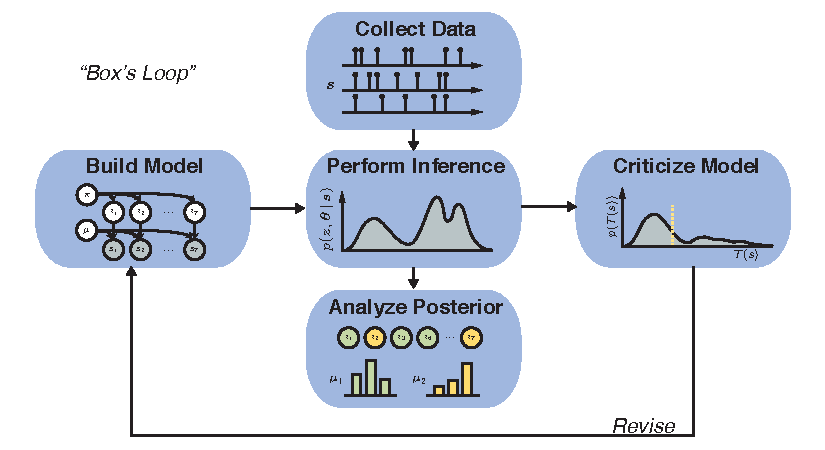
\includegraphics[width=5.5in]{figures/ch1/boxloop} 
\caption[Box's Loop]{Box's loop for hypothesis driven probabilistic modeling.
Adapted from~\citet{blei2014build}.}
\label{fig:boxloop}
\end{figure}

Putting this all together, 
Figure~\ref{fig:boxloop} outlines the iterative process of model building.
We begin by collecting data, in this case, large-scale recordings of neural
spike trains, and building a probabilistic model that captures our 
intuitions and hypotheses about structure in that data. Given these two 
ingredients, we perform Bayesian inference to compute the posterior 
distribution over structural variables and parameters. Visualizing, analyzing, and 
exploring this posterior often lead to new insights and ways to think 
about generative processes that can explain the data. We can also 
criticize the model, formally, by assessing goodness-of-fit, evaluating 
predictive likelihoods, and performing posterior predictive checks 
\citep{Gelman13}. This too leads to new hypotheses, which in turn lead to 
new models and another iteration of this process.
\citet{blei2014build}, from whom this
figure has been adapted, calls this ``Box's loop,'' a reference to the 
foundational work of~\citet{box1980sampling}. 



We are certainly not the first to adopt a Bayesian approach to modeling 
of neural data. Indeed, probabilistic methods \citep[e.g.]{brillinger1976identification,
Brillinger-1988, Paninski-2004, Truccolo-2005, Pillow-2008}, 
particularly Bayesian methods \citep[e.g.]{sahani1999latent, rieke1999spikes, Yu09,
park2011bayesian, macke2011empirical}, 
have played a major role in advancing our understanding of spike trains. 
We build on this foundation and specifically focus on expanding the 
set of models, combining standard point process and spike count models with 
hierarchical prior distributions that capture latent structure. To go 
along with these more sophisticated models, we also derive efficient 
Bayesian inference algorithms that take advantage of clever data augmentation 
strategies. Together, these expand the repertoire of probabilistic models 
that we can leverage when looking for structure in neural data.


\section{Summary of Contributions}

Chapter \ref{chap:two} provides a brief overview of point processes, 
probabilistic modeling, and Bayesian inference that lays the foundation for the 
methodological contributions in the remainder of the thesis. We also introduce 
common notation for spike trains, firing rates, and latent variables of the model. 
Readers who are well versed in probabilistic modeling may skip this chapter without 
much harm. 

Chapter \ref{chap:three} introduces our first probabilistic model for neural 
spike trains --- a combination of continuous time Hawkes processes and probabilistic network 
models. This is based on \citet{linderman2014discovering}. However, since this 
is the first model of the chapter, we provide a 
more thorough discussion of network models, Hawkes processes, and the steps 
in deriving an efficient Markov Chain Monte Carlo (MCMC) inference algorithm.
This is also the only chapter that will apply these techniques to spike trains 
from other domains, specifically, from social network analysis and criminology.

Chapter \ref{chap:four} continues to focus on Hawkes processes and networks, 
but here we break from the continuous time models of Chapter~\ref{chap:three} and 
begin working in discrete time. The remainder of the thesis will do the same. 
We also introduce a scalable variational inference algorithm that leverages 
the discrete model structure. This is based on \citet{linderman2015scalable}. 

Chapter~\ref{chap:five} reconsiders the linear interactions of Hawkes processes 
and develops a nonlinear autoregressive model for neural spike trains. Again, 
we use probabilistic network models as prior distributions over the pattern of 
functional interaction, and in doing so, we show that interesting representations 
of neural populations can be learned directly from the data. A preliminary version 
of this work was presented by \citet{linderman2015cosyne}.

Chapter~\ref{chap:six} continues on the network theme, but here we begin to 
transition from static models to ones with dynamic latent states. Specifically, 
we adopt a mechanistic view of the network and treat its connections as actual
synapses. From this perspective, it is natural to consider dynamic learning rules 
that govern how synaptic weights evolve over time. We derive a framework for 
modeling arbitrary synaptic plasticity rules and fitting them with particle MCMC.
This chapter is based on \citet{linderman2014framework}.

Chapter~\ref{chap:seven} departs from network models and instead considers 
dynamical state space models, specifically Hidden Markov Models (HMM), for 
neural data. We address a major challenge in applying these well-known models ---
deciding the number of latent states. We develop a Bayesian nonparametric model 
by introducing a hierarchical Dirichlet process (HDP) prior and both an MCMC 
and a variational inference algorithm. While this 
combination is relatively well studied, these models are notoriously 
sensitive to hyperparameter settings. We introduce a variety of methods for 
selecting hyperparameters and perform a thorough comparison on real and synthetic 
data. This is based on \citet{linderman2016nonparametric}.

Chapter~\ref{chap:nine} is a first step in a very novel direction. We build on 
the probabilistic models of the preceding chapters, but here we combine these 
models with a top-down theory of neural computation. Specifically, we consider 
the repercussions of the ``Bayesian brain'' hypothesis, namely, that neural 
circuits are performing approximate Bayesian inference in a probabilistic model
of the world. We make predictions about the patterns of neural
spike trains would be expected from such a circuit, and we show how the methods 
of previous chapters can be leveraged to reverse engineer probabilistic models 
from observations of neural spike trains. This work is necessarily speculative, 
but we believe it suggests a promising path forward as we seek to reconcile 
computational and algorithmic theories of neural computation with large scale 
recordings. 


